\documentclass{article}
\usepackage{../fasy-hw}

%% UPDATE these variables:
\renewcommand{\hwnum}{3}
\title{Discrete Structures, Homework \hwnum}
\author{Braeden Hunt (Tinnittin)}
\collab{n/a}
\date{due: 19 February 2021}

\begin{document}

\maketitle

This homework assignment should be
submitted as a single PDF file both to D2L and to Gradescope.

General homework expectations:
\begin{itemize}
    \item Homework should be typeset using LaTex.
    \item Answers should be in complete sentences and proofread.
    \item You will not plagiarize.  \item List collaborators at the start of each question using the \texttt{collab} command.
    \item Put your answers where the \texttt{todo} command currently is (and
        remove the \texttt{todo}, but not the word \texttt{Answer}).
\end{itemize}

% ============================================
% ============================================
\collab{n/a} \nextprob{Negations}
% ============================================
% ============================================
Negate the following statements:

\begin{enumerate}

    \item Each ``Clean 'Cat Kit''  contains a cloth mask and a refillable hand
        sanitizer.

        \paragraph{Answer}
        There exists a ```Clean `Cat Kit'' that does not contain a cloth mask or does not contain a refillable and sanitizer.

    \item There exists a boat docked in New Jersey that I have steered.

        \paragraph{Answer}
        For all boats docked in New Jersey, I have not steered them.

    \item There exists an island in the Ohio River with a bowling alley and a
        university track field.

        \paragraph{Answer}
        For all islands x in the Ohio River, x does not have a bowling alley or does not have a university track field.

    \item Both my sister and I can climb every route at Spire.

        \paragraph{Answer}
	There exists a route at Spire that either my sister can't climb or I can't climb.

\end{enumerate}

% ============================================
% ============================================
\collab{n/a} \nextprob{Definitions}
% ============================================
% ============================================
Use the definitions provided in the course textbook to prove that every prime
number except~$2$ is odd.

\paragraph{Answer}

For every prime number $p$, $p > 1$, and if $p = rs$ where $r$ and $s$ are both positive integers, either $r$ or $s$ is equal to $p$ and the other is equal to 1.
Every even number $e$ can be written as $e = 2k$ where $k$ is some integer. 
Using these definitions, for a number $x$ to be both prime and even, $x = 2k$ and $x = rs$ where $r$ or $s$ has to equal $x$.
We can substitute these and see that $2k = rs$.
Since we know that one of $r$ or $s$ has to equal to $x$, we know that one of them is 2 and the other is 1. Therefore, the only solution to a number being both even and prime is 2.
%
% ============================================
% ============================================
\collab{n/a}
\nextprob{Four Colors Suffice}
% ============================================
% ============================================
Read Chapters $2$ and $3$ of \emph{Four Colors Suffice} and answer the following questions:

\begin{enumerate}

    \item Who are the Austrian(s) mentioned in Chapters $1$--$3$, and what was their
        contribution mentioned in the book?

        \paragraph{Answer}
        Heinrich Tietze extended the four color problem and the 
        5 princes problem into the third dimension. He showed that in 3 dimensions, you 
        could have maps that required infinitely many colors as it is possible to construct 
        maps out of flexible rods such that every rod touches every other rod. He also restated
        the 5 prince problem so that they needed to connect non-crossing roads to each palace
        rather than bordering territories, which is in effect, the same problem. He also offered a
        ``solution'' to the problem by extending it off the planar surface (onto a torus) by 
        connecting roads or territories with bridges.

    \item Write a statement of the four color theorem using a universal
        quantifier.

        \paragraph{Answer}
        For each map $m$, $m$'s regions can be labeled such that no two regions that share a border have the same label by using at most four labels.

    \item What is the definition of a $k$-coloring of a graph?

        \paragraph{Answer}
        A $k$-coloring of a graph is one possible way of coloring a graph's vertices with k colors such that no two connected vertices have the same color.

    \item Prove or disprove: all planar graphs are three-colorable.

        \paragraph{Answer}
        Figure \ref{4colors} shows a graph that cannot be colored with only three colors, disproving the statement via counterexample.
\begin{figure}
\caption{4 Color Map}
\centering
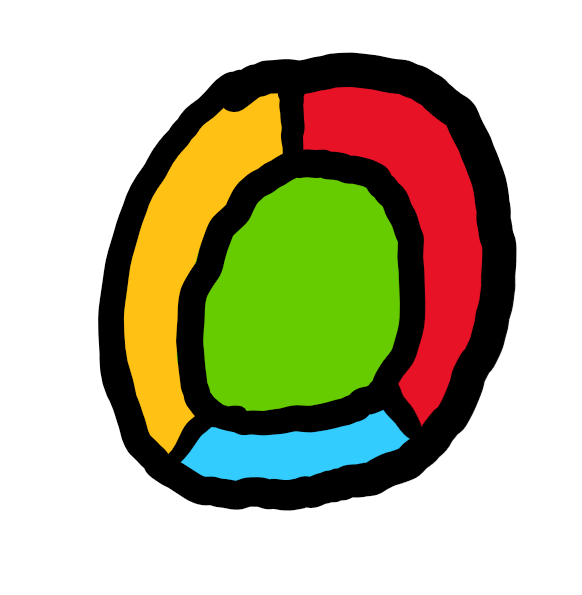
\includegraphics[width=0.5\textwidth]{images/4 colors}
\label{4colors}
\end{figure}

    \item Assuming the four color theorem holds, prove or disprove: six colors
        suffice to color a plane graph.

        \paragraph{Answer}
        p = $m$ can be colored with 4 or less colors.
        
        q = $m$ can be colored with 6 or less colors.
        
        Statement: For all maps $m$, if $p$, then $q$.
        
        If a map can be colored with 1, 2, 3, or 4 colors, then $p$.
        
        If a map can be colored with 1, 2, 3, 4, 5, or 6 colors, then $q$.
        
        By substitution, if $p$ or 5 or 6 colors, then $q$.
        
        Since $p$ is assumed true, the condition is a tautology. Through Modus Ponens, $q$ is true;
        
        Therefore, six colors suffice to color a plane graph.


    \item Give an example of a map with at least five faces that has a
        two-coloring.  Be sure to provide a coloring as evidence that the map is
        two-colorable.

        \paragraph{Answer}
        See Figure \ref{5face}.
 \begin{figure}
\caption{5 Face, 2 Color Map}
\centering
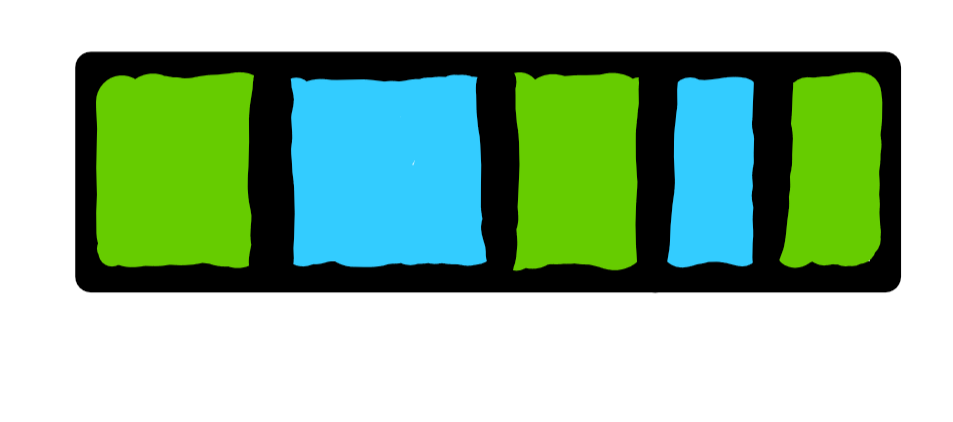
\includegraphics[width=0.5\textwidth]{images/5 face}
\label{5face}
\end{figure}

    \item Euler's formula states that if we have a map on the sphere or plane
        and count the exterior face as a face, then F-E+V=2.  Does this equation
        hold if the map is drawn on a M\"obius band? Why or why not? (Note:
        here, the boundary of the M\"obius band must be represented in the graph
        defining the map, and no ``country'' can be on the same side of a single
        edge.)

        \paragraph{Answer}
        It does not. For example, if we have a map of only one region on a M\"obius band, 
        we have 1 face, 1 edge, and no vertices. Substituting those values into Euler's formula,
         we get $1-1+0=2$ or $0=2$, which is not true. Therefore, Euler's formula does not hold up.

    \item In your own words, explain the joke: ``A topologist cannot tell the
        difference between a coffee cup and a donut.''  You are encouraged to
        use Wikipedia to formulate your answer, but be sure to cite sources.

        \paragraph{Answer}
        In topology, a coffee mug and a donut are the same basic shape, a torus. 
        They are considered the same shape because one can be modeled into the 
        other without loosing its core properties. Imagine you have a donut made of
        clay. You are able to model it into a coffee mug without putting a hole through
        it or joining faces/ends together. Therefore, to a topologist, they are the same shape.
        
        Source: \url{https://phys.org/news/2016-10-coffee-donut-topology.html} and 
        some personal experience with 3D modeling.

\end{enumerate}

% ============================================
% ============================================
\collab{n/a}
\nextprob{Ada Lovelace}
% ============================================
% ============================================

Write a short (1-2 paragraph) biography of Ada Lovelace.
\textbf{In your own words}, describe who they are and why they are important in
the history of computer science.  If you use external resources, please provide
proper citations (see the `hw/bib-ex` folder for examples of how to use
citations). If you do not use external sources, please write ``I did not
use any sources to write this biography'' as the last sentence of the
biography.

\paragraph{Answer}

Ada Lovelace was an English Aristocrat who was forced to study 
math and science from a very young age by her mother. Her study 
of mathematics eventually led her to meeting Charles Babbage, who 
is known as the father of computing. While translating articles about
Babbage's designs and inventions, she added her own thoughts to them.
She came up with new concepts such as looping and she developed algorithms.
Because of this, she is considered the first computer programmer.

Source: \url{biography.com/scholar/ada-lovelace}

% %% ... the bibliography
% \newpage
% \bibliographystyle{acm}
% \bibliography{biblio}

\end{document}

